% !TeX program = lualatex
% ================================================================
% Polish Parallel Text Version of CollectingAndMultiplyingTerms
%
% Generated by the server using the following settings:
%
%   language            Polish (pol)
%   text direction      left to right
%   font                Noto Serif
%   fallback font       Noto Serif
%   built from          latex/worksheets/algebra/collectingAndMultiplyingTerms.tex
%   vocabulary key      latex/worksheets/algebra/collectingAndMultiplyingTerms/L2/pol/collectingAndMultiplyingTerms_polishKey.tex
%   tier 3 vocabulary   green   RGB 0 128 0
%   English text        black   RGB 0 0 0
%   Polish text         purple  RGB 112 48 160
%   layout macros       version 3
%
% Please don't edit any information in this comment block - the server
% compares it against the current settings and rebuilds this file when
% they differ, so changes here would be overwritten. However, feel free
% to make updates to the LaTeX below if you want to edit it.
% ================================================================

\documentclass[12pt,a4paper]{article}
% ================================================================
% Copied from the English sheet this was translated from, so that
% anything it sets up for itself still works here
% ================================================================
\usepackage[a4paper,top=12mm,bottom=12mm,left=14mm,right=14mm]{geometry}
\usepackage[T1]{fontenc}
\usepackage{amsmath}
\usepackage{amssymb}
% A sans serif font with a single-storey a, as children write it. It is
% used for the mathematics as well as the text.
\usepackage{tgadventor}
\renewcommand*{\familydefault}{\sfdefault}
\usepackage[italic]{mathastext}
\usepackage{multicol}
\usepackage{tikz}
\usepackage[most]{tcolorbox}
\usetikzlibrary{arrows.meta}

% ================================================================
% Collecting and multiplying terms: a drill booklet that follows the
% algebraic terminology sheet.
%
% Each page practises one kind of simplification, and each page is a
% small step on from the one before:
%
%   1  adding terms in one variable
%   2  subtracting terms in one variable
%   3  collecting like terms, all positive
%   4  collecting like terms with subtraction (the sign belongs to
%      the term)
%   5  collecting like terms where a coefficient comes out negative
%   6  multiplying terms
%   7  multiplying terms with negative coefficients
%   8  multiplying a variable by itself: squares and cubes
%   9  multiplying powers of one variable
%  10  multiplying powers of more than one variable
%  11  collecting like terms with powers
%  12  multiplying, then collecting like terms
%  13  problem solving
%
% Pages 1 to 12 have the same three parts. A worked example shows the
% method, with a note beside it saying why it works. Then two questions
% repeat the worked example's layout line for line, the first with
% most of the working given and the second with only the words given,
% so that the support is taken away in two steps. Then there is a list
% of questions in two columns that starts easier than the worked
% example and finishes a little harder.
%
% The answers are in a comment beside each question.
% ================================================================

\pagestyle{empty}
\setlength{\parindent}{0pt}
\setlength{\parskip}{0pt}
\setlength{\columnsep}{8mm}
\setlength{\multicolsep}{4pt}
% Ragged right, so that the spaces between words are all the same.
\AtBeginDocument{\raggedright}

% The worked examples and the key idea, in boxes that are tinted only
% faintly, so that the sheet is cheap to print.
\newtcolorbox{keyidea}{colback=orange!3,colframe=orange!35,boxrule=0.6pt,
  left=6pt,right=6pt,top=4pt,bottom=4pt,before upper=\raggedright}
\newtcolorbox{wex}{colback=blue!2,colframe=blue!30,boxrule=0.6pt,
  colbacktitle=blue!8,coltitle=blue!50!black,
  left=6pt,right=6pt,top=2pt,bottom=4pt,before upper=\raggedright,
  title={\bfseries Worked example},toptitle=1pt,bottomtitle=1pt}

% The title of a page. The questions are numbered from 1 again on each
% page, so that a question can be found from its page and its number.
\newcommand{\topic}[1]{\setcounter{qnum}{0}{\Large\bfseries #1}\par\vspace{6pt}}

% An instruction for the questions after it.
\newcommand{\instruction}[1]{\par\vspace{10pt}{\bfseries #1}\par\vspace{2pt}}

% Gaps to write in: \gap for a term, \wgap for a longer term or a short
% expression, and \lgap for a long expression. The strut keeps the
% lines far enough apart to write on.
\newcommand{\gapstrut}{\rule[-1.8mm]{0pt}{8mm}}
\newcommand{\gap}{\gapstrut\underline{\hspace{1.5cm}}}
\newcommand{\wgap}{\gapstrut\underline{\hspace{2.6cm}}}
\newcommand{\lgap}{\gapstrut\underline{\hspace{4.2cm}}}
% A gap for an index. An underline sits too low to be read as an index,
% so a faint dotted box marks where the number is written.
\newcommand{\boxgap}{\tikz[baseline=-0.8pt]\draw[gray!60,densely dotted,thick]
  (0,0) rectangle (8pt,8pt);}

% The method, set out one line at a time. The worked example and the
% two questions after it all use this width, so that their lines break
% in the same places and the layouts match line for line.
\newlength{\workwidth}\setlength{\workwidth}{7.7cm}
\newlength{\qlabelwidth}\setlength{\qlabelwidth}{1.1cm}
\newenvironment{working}
  {\begin{minipage}[t]{\workwidth}\raggedright\everypar{\gapstrut}}
  {\end{minipage}}
% The note beside the working, in the rest of the worked example box.
\newenvironment{wexnote}
  {\hfill\begin{minipage}[t]{\dimexpr\linewidth-\workwidth-6mm\relax}%
   \raggedright\vspace{4pt}\setlength{\parskip}{5pt}}
  {\end{minipage}}

% The question number. A question that runs onto a second line is
% indented to line up with its first line.
\newcounter{qnum}
\newcommand{\qlabel}{\stepcounter{qnum}\hangindent=\qlabelwidth\hangafter=1
  \makebox[\qlabelwidth][l]{\textbf{Q\theqnum.}}}

% A question that repeats the worked example with gaps in it. Two of
% them sit side by side.
\newenvironment{scaffold}
  {\begin{minipage}[t]{0.49\linewidth}\qlabel\begin{working}}
  {\end{working}\end{minipage}}

% The list of questions, in two columns. Each question is a term or an
% expression to simplify, then an answer line to the end of the column.
% \sq is for a short question, and \sql puts the answer line on a line
% of its own, for a long one. (TeX removes glue from the end of a
% paragraph, so a \kern follows the line to keep it.)
\newenvironment{questions}
  {\begin{multicols}{2}\raggedright}
  {\end{multicols}}
\newcommand{\ansline}{\nobreak\hspace{2pt}\gapstrut
  \leaders\hrule\hskip 2.8cm plus 1fill\kern0pt\par}
\newcommand{\sq}[1]{\par\qlabel$#1={}$\ansline\vspace{7pt}}
\newcommand{\sql}[1]{\par\qlabel$#1$\par
  \hspace*{\qlabelwidth}$={}$\ansline\vspace{7pt}}

% A line to write a sentence on, the width of the column.
\newcommand{\writeline}{\par\gapstrut\leaders\hrule\hskip 0pt plus 1fill\kern0pt\par}

% A box for a missing term.
\newcommand{\missing}{\tikz[baseline=-4pt]\draw[thick] (0,-0.25) rectangle (1.5,0.55);}

% Characters this language's font has not got are borrowed from another,
% rather than being silently dropped - see docs/translated-sheet-latex.md
\directlua{%
  if luaotfload and luaotfload.add_fallback then
    luaotfload.add_fallback("eallatinfallback",
      { "Noto Serif:mode=harf;" })
  else
    tex.error("this luaotfload is too old to register a fallback font")
  end
}
\usepackage[english]{babel}
\babelprovide[import]{polish}
\babelfont[polish]{rm}[Renderer=Harfbuzz, BoldFont={Noto Serif}, ItalicFont={Noto Serif}, BoldItalicFont={Noto Serif}, RawFeature={fallback=eallatinfallback}]{Noto Serif}
\babelfont[polish]{sf}[Renderer=Harfbuzz, BoldFont={Noto Serif}, ItalicFont={Noto Serif}, BoldItalicFont={Noto Serif}, RawFeature={fallback=eallatinfallback}]{Noto Serif}
\newcommand{\ealtext}[1]{\foreignlanguage{polish}{#1}}
\newcommand{\ealtextblock}[1]{{\raggedright\foreignlanguage{polish}{#1}\par}}
% ================================================================
% EAL layout helpers
% ================================================================
\usepackage{xcolor}

\definecolor{ealkeycolour}{RGB}{0,128,0}
\definecolor{ealenglish}{RGB}{0,0,0}
\definecolor{ealtwocolour}{RGB}{112,48,160}

\newsavebox{\ealboxen}
\newsavebox{\ealboxtr}
\newlength{\ealglosswd}
\newlength{\ealglossraise}
\setlength{\ealglossraise}{1.15em}

% a tier 3 word, in English and in translation alike
\newcommand{\ealkey}[1]{\textcolor{ealkeycolour}{#1}}
\newcommand{\ealkeytr}[1]{\textcolor{ealkeycolour}{\ealtext{#1}}}

% One translated word above one English word. Built from kernel
% primitives, never a tabular, which would break wherever the sheet
% loads array, booktabs or tabularx. The box is as wide as the wider of
% the two, so a long translation pushes its neighbours aside instead of
% overlapping them, and it claims its full height so a table row or a
% TikZ node makes room for it.
\newcommand{\ealgloss}[2]{%
  \sbox{\ealboxen}{\ealkey{#1}}%
  \sbox{\ealboxtr}{\small\textcolor{ealtwocolour}{\ealtext{#2}}}%
  \setlength{\ealglosswd}{\wd\ealboxen}%
  \ifdim\wd\ealboxtr>\ealglosswd\setlength{\ealglosswd}{\wd\ealboxtr}\fi
  \leavevmode
  \makebox[\ealglosswd][c]{%
    \makebox[0pt][c]{\usebox{\ealboxen}}%
    \makebox[0pt][c]{\raisebox{\ealglossraise}{\usebox{\ealboxtr}}}%
  }%
}

% opens up line spacing around a block of glosses, so the raised
% translations sit clear of the line above
\newenvironment{ealglossed}{\par\linespread{2.1}\selectfont\ignorespaces}{\par}

% a whole translated sentence above its English counterpart. block level,
% so it does not belong inside a tabular cell
\newcommand{\ealpara}[2]{%
  \par\addvspace{0.5\baselineskip}%
  {\color{ealtwocolour}\ealtextblock{#1}}%
  \penalty200
  {\color{ealenglish}#2\par}%
  \addvspace{0.5\baselineskip}%
}

\begin{document}

\ealpara{Redukowanie i mnożenie \ealkeytr{wyrazów}}{\ealkey{Collecting} and Multiplying \ealkey{Terms}}
\begin{center}
  {\LARGE\bfseries \ealkey{Collecting} and Multiplying \ealkey{Terms}}
\end{center}
\vspace{-6pt}

\begin{keyidea}
\ealpara{\ealkeytr{Wyraz} to liczba, \ealkeytr{zmienna}, albo liczby i \ealkeytr{zmienne} pomnożone razem. \ealkeytr{Współczynnik} \ealkeytr{wyrazu} to liczba, która mnoży \ealkeytr{zmienne} w nim.}{A \textbf{\ealkey{term}} is a number, a \textbf{\ealkey{variable}}, or numbers and \ealkey{variables} multiplied together. The \textbf{\ealkey{coefficient}} of a \ealkey{term} is the number that multiplies the \ealkey{variables} in it.}

\vspace{3pt}
\ealpara{Aby \ealkeytr{uprościć} \ealkeytr{wyrażenie}, zapisujemy je w krótszy sposób, równy mu dla każdej wartości \ealkeytr{zmiennych}. Prześledź rozwiązane przykłady w tej książeczce, aby nauczyć się, jak \ealkeytr{uprościć} \ealkeytr{wyrażenia}.}{To \textbf{\ealkey{simplify}} an \textbf{\ealkey{expression}}, we write it in a shorter way that is equal to it for every value of the \ealkey{variables}. Follow the worked examples in this booklet to learn how to \ealkey{simplify} \ealkey{expressions}.}
\end{keyidea}

\vspace{6pt}
\ealpara{1. Dodawanie \ealkeytr{wyrazów}}{1. Adding \ealkey{terms}}
\topic{1. Adding \ealkey{terms}}

\begin{wex}
\begin{working}
\ealpara{Uprość $3a+2a$.}{\ealkey{Simplify} $3a+2a$.}

\ealpara{$3a$ oznacza $a+a+a$.}{$3a$ means $a+a+a$.}

\ealpara{$2a$ oznacza $a+a$.}{$2a$ means $a+a$.}

$3a+2a=a+a+a+a+a$

\ealpara{Zatem $3a+2a=5a$.}{So $3a+2a=5a$.}
\end{working}
\begin{wexnote}
\ealpara{$3a$ oznacza $3\times a$, czyli $a+a+a$. \ealkeytr{Współczynnik} $3a$ wynosi $3$.}{$3a$ means $3\times a$, which is $a+a+a$. The \ealkey{coefficient} of $3a$ is $3$.}

\ealpara{W $3a+2a$ \ealkeytr{zmienna} $a$ jest dodana $3+2=5$ razy. Aby dodać \ealkeytr{wyrazy}, dodajemy ich \ealkeytr{współczynniki}.}{In $3a+2a$, the \ealkey{variable} $a$ is added $3+2=5$ times. So to add the \ealkey{terms}, we add their \ealkey{coefficients}.}

\ealpara{\ealkeytr{Zmienna} sama w sobie ma \ealkeytr{współczynnik} $1$: $b$ oznacza $1b$. Zatem $b+2b=3b$. Piszemy $b$, a nie $1b$.}{A \ealkey{variable} on its own has a \ealkey{coefficient} of $1$: $b$ means $1b$. So $b+2b=3b$. We write $b$, not $1b$.}
\end{wexnote}
\end{wex}

\ealpara{Uzupełnij luki.}{Fill in the gaps.}
\instruction{Fill in the gaps.}

% Answers: b+b+b; 7b.
\begin{scaffold}
\ealpara{Uprość $4b+3b$.}{\ealkey{Simplify} $4b+3b$.}

\ealpara{$4b$ oznacza $b+b+b+b$.}{$4b$ means $b+b+b+b$.}

\ealpara{$3b$ oznacza \ldots}{$3b$ means \wgap.}

$4b+3b=b+b+b+b+b+b+b$

\ealpara{Zatem $4b+3b=$ \ldots}{So $4b+3b=$ \gap.}
\end{scaffold}\hfill
% Answers: x+x; x+x+x+x+x; x+x+x+x+x+x+x; 7x.
\begin{scaffold}
\ealpara{Uprość $2x+5x$.}{\ealkey{Simplify} $2x+5x$.}

\ealpara{$2x$ oznacza \ldots}{$2x$ means \wgap.}

\ealpara{$5x$ oznacza \ldots}{$5x$ means \lgap.}

$2x+5x=$ \lgap

\ealpara{Zatem $2x+5x=$ \ldots}{So $2x+5x=$ \gap.}
\end{scaffold}

\ealpara{\ealkeytr{Uprość}.}{\ealkey{Simplify}.}
\instruction{\ealkey{Simplify}.}

\begin{questions}
\sq{5a+2a}        % 7a
\sq{3b+4b}        % 7b
\sq{6x+3x}        % 9x
\sq{2y+8y}        % 10y
\sq{4m+4m}        % 8m
\sq{7p+5p}        % 12p
\sq{a+4a}         % 5a
\sq{9t+t}         % 10t
\sq{c+c}          % 2c
\sq{10n+6n}       % 16n
\sq{2a+3a+4a}     % 9a
\sq{5k+k+6k}      % 12k
\sq{x+x+x+x}      % 4x
\sq{12y+15y}      % 27y
\sq{3d+2d+d+4d}   % 10d
\sq{20z+13z+7z}   % 40z
\end{questions}

\newpage
% ================================================================
% PAGE 2: subtracting terms in one variable
% ================================================================

\ealpara{2. Odejmowanie \ealkeytr{wyrazów}}{2. Subtracting \ealkey{terms}}
\topic{2. Subtracting \ealkey{terms}}

\begin{wex}
\begin{working}
\ealpara{Uprość $8a+3a-5a$.}{\ealkey{Simplify} $8a+3a-5a$.}

\ealpara{Pracujemy od lewej do prawej.}{We work from left to right.}

$8a+3a=11a$

$11a-5a=6a$

\ealpara{Zatem $8a+3a-5a=6a$.}{So $8a+3a-5a=6a$.}
\end{working}
\begin{wexnote}
\ealpara{Aby odjąć \ealkeytr{wyrazy} z tą samą \ealkeytr{zmienną}, odejmujemy ich \ealkeytr{współczynniki}: $11-5=6$.}{To subtract \ealkey{terms} with the same \ealkey{variable}, we subtract their \ealkey{coefficients}: $11-5=6$.}

\ealpara{Gdy są więcej niż dwa \ealkeytr{wyrazy}, pracujemy od lewej do prawej, po jednym \ealkeytr{wyrazie} na raz.}{When there are more than two \ealkey{terms}, we work from left to right, one \ealkey{term} at a time.}

\ealpara{Gdy \ealkeytr{współczynnik} wynosi $1$, piszemy $a$, a nie $1a$. Gdy \ealkeytr{współczynniki} \ealkeytr{skrócą się}, odpowiedź wynosi $0$: $4a-4a=0$.}{When the \ealkey{coefficient} is $1$, we write $a$, not $1a$. When the \ealkey{coefficients} \ealkey{cancel out}, the answer is $0$: $4a-4a=0$.}
\end{wexnote}
\end{wex}

\ealpara{Uzupełnij luki.}{Fill in the gaps.}
\instruction{Fill in the gaps.}

% Answers: 7b; 7b.
\begin{scaffold}
\ealpara{Uprość $6b+4b-3b$.}{\ealkey{Simplify} $6b+4b-3b$.}

\ealpara{Pracujemy od lewej do prawej.}{We work from left to right.}

$6b+4b=10b$

$10b-3b=$ \gap

\ealpara{Zatem $6b+4b-3b=$ \ldots}{So $6b+4b-3b=$ \gap.}
\end{scaffold}\hfill
% Answers: 7x; 7x + 5x = 12x; 12x.
\begin{scaffold}
\ealpara{Uprość $9x-2x+5x$.}{\ealkey{Simplify} $9x-2x+5x$.}

\ealpara{Pracujemy od lewej do prawej.}{We work from left to right.}

$9x-2x=$ \gap

\gap\ $+\,5x=$ \gap

\ealpara{Zatem $9x-2x+5x=$ \ldots}{So $9x-2x+5x=$ \gap.}
\end{scaffold}

\ealpara{\ealkeytr{Uprość}.}{\ealkey{Simplify}.}
\instruction{\ealkey{Simplify}.}

\begin{questions}
\sq{7a-3a}          % 4a
\sq{9b-4b}          % 5b
\sq{10x-6x}         % 4x
\sq{8y-y}           % 7y
\sq{12m-5m}         % 7m
\sq{14q-8q}         % 6q
\sq{11h-h}          % 10h
\sq{5p-4p}          % p
\sq{6t-6t}          % 0
\sq{20n-9n}         % 11n
\sq{25w-17w}        % 8w
\sq{4a+6a-3a}       % 7a
\sq{5k+k-2k}        % 4k
\sq{9a+a-4a}        % 6a
\sq{8b+2b-7b}       % 3b
\sq{9p-2p+4p}       % 11p
\sq{6r-4r+5r}       % 7r
\sq{12t-5t-2t}      % 5t
\sq{10g-3g-3g}      % 4g
\sq{x+7x-3x}        % 5x
\sq{10c-4c-6c}      % 0
\sq{8y-3y+2y-4y}    % 3y
\sq{7m+m-5m+2m}     % 5m
\sq{15d-7d+d-8d}    % d
\end{questions}

\newpage
% ================================================================
% PAGE 3: collecting like terms, all positive
% ================================================================

\ealpara{3. \ealkeytr{Redukowanie} \ealkeytr{wyrazów podobnych}}{3. \ealkey{Collecting} \ealkey{like terms}}
\topic{3. \ealkey{Collecting} \ealkey{like terms}}

\begin{wex}
\begin{working}
\ealpara{Uprość $5a+3b+2a+4b$.}{\ealkey{Simplify} $5a+3b+2a+4b$.}

\ealpara{\ealkeytr{Wyrazy podobne} to $5a$ i $2a$ oraz $3b$ i $4b$.}{The \ealkey{like terms} are $5a$ and $2a$, and $3b$ and $4b$.}

$5a+2a=7a$

$3b+4b=7b$

\ealpara{Zatem $5a+3b+2a+4b=7a+7b$.}{So $5a+3b+2a+4b=7a+7b$.}
\end{working}
\begin{wexnote}
\ealpara{\ealkeytr{Wyrazy podobne} mają dokładnie takie same \ealkeytr{zmienne}. $5a$ i $2a$ to \ealkeytr{wyrazy podobne}, a $3b$ i $4b$ to \ealkeytr{wyrazy podobne}.}{\textbf{\ealkey{Like terms}} have exactly the same \ealkey{variables}. $5a$ and $2a$ are \ealkey{like terms}, and $3b$ and $4b$ are \ealkey{like terms}.}

\ealpara{\ealkeytr{Redukujemy} każdy zestaw \ealkeytr{wyrazów podobnych} do jednego \ealkeytr{wyrazu}.}{We \ealkey{collect} each set of \ealkey{like terms} into a single \ealkey{term}.}

\ealpara{$7a$ i $7b$ nie są \ealkeytr{wyrazami podobnymi}, więc $7a+7b$ nie można \ealkeytr{uprościć}.}{$7a$ and $7b$ are not \ealkey{like terms}, so $7a+7b$ cannot be \ealkey{simplified}.}

\ealpara{\ealkeytr{Stałe} są \ealkeytr{wyrazami podobnymi} względem siebie: $4+2=6$.}{\ealkey{Constants} are \ealkey{like terms} with each other: $4+2=6$.}
\end{wexnote}
\end{wex}

\ealpara{Uzupełnij luki.}{Fill in the gaps.}
\instruction{Fill in the gaps.}

% Answers: 2y and 5y; 7x; 7y; 7x + 7y.
\begin{scaffold}
\ealpara{Uprość $4x+2y+3x+5y$.}{\ealkey{Simplify} $4x+2y+3x+5y$.}

\ealpara{\ealkeytr{Wyrazy podobne} to $4x$ i $3x$ oraz \ldots\ i \ldots}{The \ealkey{like terms} are $4x$ and $3x$, and \gap\ and \gap.}

$4x+3x=$ \gap

$2y+5y=$ \gap

\ealpara{Zatem $4x+2y+3x+5y=$ \ldots}{So $4x+2y+3x+5y=$ \wgap.}
\end{scaffold}\hfill
% Answers: 2m and m, and 6n and 3n; 2m + m = 3m; 6n + 3n = 9n;
% 3m + 9n.
\begin{scaffold}
\ealpara{Uprość $2m+6n+m+3n$.}{\ealkey{Simplify} $2m+6n+m+3n$.}

\ealpara{\ealkeytr{Wyrazy podobne} to \ldots\ i \ldots, oraz \ldots\ i \ldots}{The \ealkey{like terms} are \gap\ and \gap, and \gap\ and \gap.}

\gap\ $+$ \gap\ $=$ \gap

\gap\ $+$ \gap\ $=$ \gap

\ealpara{Zatem $2m+6n+m+3n=$ \ldots}{So $2m+6n+m+3n=$ \wgap.}
\end{scaffold}

\ealpara{\ealkeytr{Uprość}. Jeśli \ealkeytr{wyrażenia} nie można \ealkeytr{uprościć}, napisz „nie można \ealkeytr{uprościć}”.}{\ealkey{Simplify}. If an \ealkey{expression} cannot be \ealkey{simplified}, write ``cannot be \ealkey{simplified}''.}
\instruction{\ealkey{Simplify}. If an \ealkey{expression} cannot be \ealkey{simplified}, write ``cannot be \ealkey{simplified}''.}

\begin{questions}
\sq{3a+2b+4a}           % 7a+2b
\sq{5x+2y+3y}           % 5x+5y
\sq{4p+3p+2q}           % 7p+2q
\sq{2x+3x+4y}           % 5x+4y
\sq{2a+3b+4a+b}         % 6a+4b
\sq{6p+q+2p+5q}         % 8p+6q
\sq{3m+4n+3m+4n}        % 6m+8n
\sq{4a+5+3a}            % 7a+5
\sq{x+4+3x+2}           % 4x+6
\sq{6+3t+t}             % 4t+6
\sq{7+2m+5+m}           % 3m+12
\sq{4m+n+2+m}           % 5m+n+2
\sq{5y+1+y+8}           % 6y+9
\sq{3a+2b+6}            % cannot be simplified
\sq{a+b+a+b+a}          % 3a+2b
\sql{4c+3d+c+2d+5c}     % 10c+5d
\sql{2x+3y+4z+x+y}      % 3x+4y+4z
\sq{3ab+4a+2ab}         % 5ab+4a
\sql{6xy+2x+xy+5x}      % 7xy+7x
\sql{2k+9+3h+4+k+5h}    % 8h+3k+13
\end{questions}

\newpage
% ================================================================
% PAGE 4: collecting like terms with subtraction
% ================================================================

\ealpara{4. \ealkeytr{Redukowanie} \ealkeytr{wyrazów podobnych} z odejmowaniem}{4. \ealkey{Collecting} \ealkey{like terms} with subtraction}
\topic{4. \ealkey{Collecting} \ealkey{like terms} with subtraction}

\begin{wex}
\begin{working}
\ealpara{Uprość $7a-2b-3a+6b$.}{\ealkey{Simplify} $7a-2b-3a+6b$.}

\ealpara{\ealkeytr{Wyrazy podobne} to $+7a$ i $-3a$ oraz $-2b$ i $+6b$.}{The \ealkey{like terms} are $+7a$ and $-3a$, and $-2b$ and $+6b$.}

$7a-3a=4a$

$-2b+6b=4b$

\ealpara{Zatem $7a-2b-3a+6b=4a+4b$.}{So $7a-2b-3a+6b=4a+4b$.}
\end{working}
\begin{wexnote}
\ealpara{\ealkeytr{Znak} przed \ealkeytr{wyrazem} należy do \ealkeytr{wyrazu}. \ealkeytr{Wyrazy} $7a-2b-3a+6b$ to $+7a$, $-2b$, $-3a$ i $+6b$. Pierwszy \ealkeytr{wyraz} nie ma przed sobą \ealkeytr{znaku}, więc jest \ealkeytr{liczbą dodatnią}.}{The \ealkey{sign} in front of a \ealkey{term} belongs to the \ealkey{term}. The \ealkey{terms} of $7a-2b-3a+6b$ are $+7a$, $-2b$, $-3a$ and $+6b$. The first \ealkey{term} has no \ealkey{sign} in front of it, so it is \ealkey{positive}.}

\ealpara{Zachowujemy \ealkeytr{znak} każdego \ealkeytr{wyrazu}, gdy \ealkeytr{redukujemy} \ealkeytr{wyrazy podobne}.}{We keep each \ealkey{term}'s \ealkey{sign} when we \ealkey{collect} the \ealkey{like terms}.}

\ealpara{$-2b+6b$ równa się $6b-2b$, czyli $4b$.}{$-2b+6b$ is equal to $6b-2b$, which is $4b$.}
\end{wexnote}
\end{wex}

\ealpara{Uzupełnij luki.}{Fill in the gaps.}
\instruction{Fill in the gaps.}

% Answers: -3y and +7y; 6x; 4y; 6x + 4y.
\begin{scaffold}
\ealpara{Uprość $8x-3y-2x+7y$.}{\ealkey{Simplify} $8x-3y-2x+7y$.}

\ealpara{\ealkeytr{Wyrazy podobne} to $+8x$ i $-2x$ oraz \ldots\ i \ldots}{The \ealkey{like terms} are $+8x$ and $-2x$, and \gap\ and \gap.}

$8x-2x=$ \gap

$-3y+7y=$ \gap

\ealpara{Zatem $8x-3y-2x+7y=$ \ldots}{So $8x-3y-2x+7y=$ \wgap.}
\end{scaffold}\hfill
% Answers: +5m and -m, and +9n and -4n; 5m - m = 4m; 9n - 4n = 5n;
% 4m + 5n.
\begin{scaffold}
\ealpara{Uprość $5m+9n-m-4n$.}{\ealkey{Simplify} $5m+9n-m-4n$.}

\ealpara{\ealkeytr{Wyrazy podobne} to \ldots\ i \ldots, oraz \ldots\ i \ldots}{The \ealkey{like terms} are \gap\ and \gap, and \gap\ and \gap.}

\wgap\ $=$ \gap

\wgap\ $=$ \gap

\ealpara{Zatem $5m+9n-m-4n=$ \ldots}{So $5m+9n-m-4n=$ \wgap.}
\end{scaffold}

\ealpara{\ealkeytr{Uprość}.}{\ealkey{Simplify}.}
\instruction{\ealkey{Simplify}.}

\begin{questions}
\sq{6a+2b-4a}             % 2a+2b
\sq{5x+7y-3y}             % 5x+4y
\sq{8m-2m+3n}             % 6m+3n
\sq{9a-4a+2b}             % 5a+2b
\sq{9p+4q-2p-q}           % 7p+3q
\sq{6x+5y-x-2y}           % 5x+3y
\sq{8m-2n+3n}             % 8m+n
\sq{4a-3b-a+5b}           % 3a+2b
\sq{8p-3q-5p+7q}          % 3p+4q
\sq{10x+7-6x-3}           % 4x+4
\sq{-2y+5x+6y}            % 5x+4y
\sq{12+5k-4-2k}           % 3k+8
\sq{11k-3-4k+5}           % 7k+2
\sq{7c-5d-2c+9d}          % 5c+4d
\sql{3c+5d-2c+4d-c}       % 9d
\sq{-3+4x+8-x}            % 3x+5
\sql{6ab+2a-4ab+3a}       % 2ab+5a
\sql{5xy-2y+3xy+7y}       % 8xy+5y
\sql{9m-4n+2-3m+6n-1}     % 6m+2n+1
\sql{7x-4y+2z-3x+6y-z}    % 4x+2y+z
\end{questions}

\newpage
% ================================================================
% PAGE 5: collecting like terms with a negative coefficient in the
% answer
% ================================================================

\ealpara{5. \ealkeytr{Ujemne} \ealkeytr{współczynniki}}{5. \ealkey{Negative} \ealkey{coefficients}}
\topic{5. \ealkey{Negative} \ealkey{coefficients}}

\begin{wex}
\begin{working}
\ealpara{Uprość $3a-5b-7a+2b$.}{\ealkey{Simplify} $3a-5b-7a+2b$.}

\ealpara{\ealkeytr{Wyrazy podobne} to $+3a$ i $-7a$ oraz $-5b$ i $+2b$.}{The \ealkey{like terms} are $+3a$ and $-7a$, and $-5b$ and $+2b$.}

$3a-7a=-4a$

$-5b+2b=-3b$

\ealpara{Zatem $3a-5b-7a+2b=-4a-3b$.}{So $3a-5b-7a+2b=-4a-3b$.}
\end{working}
\begin{wexnote}
\ealpara{Gdy liczba, którą odejmujemy, jest większa od liczby, od której zaczynamy, \ealkeytr{współczynnik} jest \ealkeytr{ujemny}. Aby obliczyć $3-7$, zaczynamy od $3$ na \ealkeytr{osi liczbowej} i przesuwamy się o $7$ w lewo.}{When the number we subtract is bigger than the number we start with, the \ealkey{coefficient} is \ealkey{negative}. To work out $3-7$, we start at $3$ on the \ealkey{number line} and move $7$ to the left.}

\vspace{2pt}
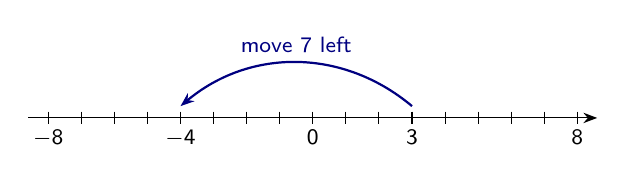
\begin{tikzpicture}[x=0.42cm]
  \draw[-{Stealth[length=5pt]}] (-8.6,0) -- (8.6,0);
  \foreach \n in {-8,...,8} \draw (\n,0.08) -- (\n,-0.08);
  \foreach \n in {-8,-4,0,3,8}
    \node[below,font=\footnotesize,inner sep=2pt] at (\n,-0.08) {$\n$};
  \draw[-{Stealth[length=5pt]},thick,blue!50!black]
    (3,0.15) to[bend right=40] node[above,font=\footnotesize] {move $7$ left} (-4,0.15);
\end{tikzpicture}

\ealpara{Zatem $3-7=-4$, i w ten sam sposób $-5+2=-3$.}{So $3-7=-4$, and in the same way $-5+2=-3$.}
\end{wexnote}
\end{wex}

\ealpara{Uzupełnij luki.}{Fill in the gaps.}
\instruction{Fill in the gaps.}

% Answers: -3n and +n; -5m; -2n; -5m - 2n.
\begin{scaffold}
\ealpara{Uprość $4m-3n-9m+n$.}{\ealkey{Simplify} $4m-3n-9m+n$.}

\ealpara{\ealkeytr{Wyrazy podobne} to $+4m$ i $-9m$ oraz \ldots\ i \ldots}{The \ealkey{like terms} are $+4m$ and $-9m$, and \gap\ and \gap.}

$4m-9m=$ \gap

$-3n+n=$ \gap

\ealpara{Zatem $4m-3n-9m+n=$ \ldots}{So $4m-3n-9m+n=$ \wgap.}
\end{scaffold}\hfill
% Answers: +p and -6p, and +2q and -8q; p - 6p = -5p; 2q - 8q = -6q;
% -5p - 6q.
\begin{scaffold}
\ealpara{Uprość $p+2q-6p-8q$.}{\ealkey{Simplify} $p+2q-6p-8q$.}

\ealpara{\ealkeytr{Wyrazy podobne} to \ldots\ i \ldots, oraz \ldots\ i \ldots}{The \ealkey{like terms} are \gap\ and \gap, and \gap\ and \gap.}

\wgap\ $=$ \gap

\wgap\ $=$ \gap

\ealpara{Zatem $p+2q-6p-8q=$ \ldots}{So $p+2q-6p-8q=$ \wgap.}
\end{scaffold}

\ealpara{\ealkeytr{Uprość}.}{\ealkey{Simplify}.}
\instruction{\ealkey{Simplify}.}

\begin{questions}
\sq{2a-5a}              % -3a
\sq{4x-9x}              % -5x
\sq{3c-8c}              % -5c
\sq{y-6y}               % -5y
\sq{-3b+b}              % -2b
\sq{-2m-4m}             % -6m
\sq{-4y-y}              % -5y
\sq{-7p+3p}             % -4p
\sq{-k-k}               % -2k
\sq{-6n+2n-3n}          % -7n
\sq{5-2n-9}             % -2n-4
\sq{3a+2b-7a}           % -4a+2b
\sq{2a-3b-5a+b}         % -3a-2b
\sq{5x-3y-8x+y}         % -3x-2y
\sql{-4p+6q+p-9q}       % -3p-3q
\sq{2-5k-7+3k}          % -2k-5
\sql{-a-b-2a+4b}        % -3a+3b
\sq{4c-3-6c-2}          % -2c-5
\sql{3xy-5x-7xy+2x}     % -4xy-3x
\sql{8-2c-11-4c+6c}     % -3
\end{questions}

\newpage
% ================================================================
% PAGE 6: multiplying terms
% ================================================================

\ealpara{6. Mnożenie \ealkeytr{wyrazów}}{6. Multiplying \ealkey{terms}}
\topic{6. Multiplying \ealkey{terms}}

\begin{wex}
\begin{working}
\ealpara{Uprość $3a\times 4b$.}{\ealkey{Simplify} $3a\times 4b$.}

$3a\times 4b=3\times 4\times a\times b$

\ealpara{Liczby: $3\times 4=12$.}{The numbers: $3\times 4=12$.}

\ealpara{\ealkeytr{Zmienne}: $a\times b=ab$.}{The \ealkey{variables}: $a\times b=ab$.}

\ealpara{Zatem $3a\times 4b=12ab$.}{So $3a\times 4b=12ab$.}
\end{working}
\begin{wexnote}
\ealpara{$3a$ oznacza $3\times a$, a $4b$ oznacza $4\times b$.}{$3a$ means $3\times a$, and $4b$ means $4\times b$.}

\ealpara{Możemy mnożyć w dowolnej kolejności, więc mnożymy liczby razem i \ealkeytr{zmienne} razem.}{We can multiply in any order, so we multiply the numbers together and the \ealkey{variables} together.}

\ealpara{Piszemy najpierw liczbę, potem \ealkeytr{zmienne} w kolejności alfabetycznej, bez \ealkeytr{znaków} $\times$: $b\times a$ zapisujemy jako $ab$.}{We write the number first, then the \ealkey{variables} in alphabetical order, with no $\times$ \ealkey{signs}: $b\times a$ is written $ab$.}
\end{wexnote}
\end{wex}

\ealpara{Uzupełnij luki.}{Fill in the gaps.}
\instruction{Fill in the gaps.}

% Answers: 10; xy; 10xy.
\begin{scaffold}
\ealpara{Uprość $2x\times 5y$.}{\ealkey{Simplify} $2x\times 5y$.}

$2x\times 5y=2\times 5\times x\times y$

\ealpara{Liczby: $2\times 5=$ \ldots}{The numbers: $2\times 5=$ \gap.}

\ealpara{\ealkeytr{Zmienne}: $x\times y=$ \ldots}{The \ealkey{variables}: $x\times y=$ \gap.}

\ealpara{Zatem $2x\times 5y=$ \ldots}{So $2x\times 5y=$ \gap.}
\end{scaffold}\hfill
% Answers: 4 x 3 x n x m; 4 x 3 = 12; n x m = mn; 12mn.
\begin{scaffold}
\ealpara{Uprość $4n\times 3m$.}{\ealkey{Simplify} $4n\times 3m$.}

$4n\times 3m=$ \lgap

\ealpara{Liczby: \ldots\ $=$ \ldots}{The numbers: \gap\ $=$ \gap.}

\ealpara{\ealkeytr{Zmienne}: \ldots\ $=$ \ldots}{The \ealkey{variables}: \gap\ $=$ \gap.}

\ealpara{Zatem $4n\times 3m=$ \ldots}{So $4n\times 3m=$ \gap.}
\end{scaffold}

\ealpara{\ealkeytr{Uprość}.}{\ealkey{Simplify}.}
\instruction{\ealkey{Simplify}.}

\begin{questions}
\sq{4\times a}             % 4a
\sq{a\times b}             % ab
\sq{3\times 2b}            % 6b
\sq{5\times 4c}            % 20c
\sq{y\times x}             % xy
\sq{5x\times 2}            % 10x
\sq{b\times 7}             % 7b
\sq{2a\times b}            % 2ab
\sq{3x\times y}            % 3xy
\sq{p\times 6q}            % 6pq
\sq{3p\times 4q}           % 12pq
\sq{6x\times 5y}           % 30xy
\sq{4a\times 4b}           % 16ab
\sq{2b\times 9a}           % 18ab
\sq{3n\times 8m}           % 24mn
\sq{7m\times 7n}           % 49mn
\sq{5t\times 4s}           % 20st
\sq{10x\times 3y}          % 30xy
\sq{4\times 2a\times b}    % 8ab
\sq{2a\times 3b\times c}   % 6abc
\sq{a\times 2b\times 3c}   % 6abc
\sq{4x\times 3yz}          % 12xyz
\sq{2xy\times 5z}          % 10xyz
\sq{3c\times 2b\times 5a}  % 30abc
\end{questions}

\newpage
% ================================================================
% PAGE 7: multiplying terms with negative coefficients
% ================================================================

\ealpara{7. Mnożenie przez liczby \ealkeytr{ujemne}}{7. Multiplying with \ealkey{negative} numbers}
\topic{7. Multiplying with \ealkey{negative} numbers}

\begin{wex}
\begin{working}
\ealpara{Uprość $-2x\times -4y$.}{\ealkey{Simplify} $-2x\times -4y$.}

$-2x\times -4y=-2\times -4\times x\times y$

\ealpara{Liczby: $-2\times -4=8$.}{The numbers: $-2\times -4=8$.}

\ealpara{\ealkeytr{Zmienne}: $x\times y=xy$.}{The \ealkey{variables}: $x\times y=xy$.}

\ealpara{Zatem $-2x\times -4y=8xy$.}{So $-2x\times -4y=8xy$.}
\end{working}
\begin{wexnote}
\ealpara{Gdy mnożymy dwie liczby o tym samym \ealkeytr{znaku}, wynik jest \ealkeytr{liczbą dodatnią}. Gdy \ealkeytr{znaki} są różne, wynik jest \ealkeytr{ujemny}.}{When we multiply two numbers with the same \ealkey{sign}, the answer is \ealkey{positive}. When the \ealkey{signs} are different, the answer is \ealkey{negative}.}

\vspace{2pt}
\begin{tabular}{@{}l@{\qquad}l@{}}
$3\times 4=12$     & $-3\times 4=-12$\\[2pt]
$-3\times -4=12$   & $3\times -4=-12$
\end{tabular}

\ealpara{$-a$ oznacza $-1\times a$, więc \ealkeytr{współczynnik} $-a$ wynosi $-1$.}{$-a$ means $-1\times a$, so the \ealkey{coefficient} of $-a$ is $-1$.}
\end{wexnote}
\end{wex}

\ealpara{Uzupełnij luki.}{Fill in the gaps.}
\instruction{Fill in the gaps.}

% Answers: -15; ab; -15ab.
\begin{scaffold}
\ealpara{Uprość $-3a\times 5b$.}{\ealkey{Simplify} $-3a\times 5b$.}

$-3a\times 5b=-3\times 5\times a\times b$

\ealpara{Liczby: $-3\times 5=$ \ldots}{The numbers: $-3\times 5=$ \gap.}

\ealpara{\ealkeytr{Zmienne}: $a\times b=$ \ldots}{The \ealkey{variables}: $a\times b=$ \gap.}

\ealpara{Zatem $-3a\times 5b=$ \ldots}{So $-3a\times 5b=$ \gap.}
\end{scaffold}\hfill
% Answers: 6 x -2 x m x n; 6 x -2 = -12; m x n = mn; -12mn.
\begin{scaffold}
\ealpara{Uprość $6m\times -2n$.}{\ealkey{Simplify} $6m\times -2n$.}

$6m\times -2n=$ \lgap

\ealpara{Liczby: \ldots\ $=$ \ldots}{The numbers: \gap\ $=$ \gap.}

\ealpara{\ealkeytr{Zmienne}: \ldots\ $=$ \ldots}{The \ealkey{variables}: \gap\ $=$ \gap.}

\ealpara{Zatem $6m\times -2n=$ \ldots}{So $6m\times -2n=$ \gap.}
\end{scaffold}

\ealpara{\ealkeytr{Uprość}.}{\ealkey{Simplify}.}
\instruction{\ealkey{Simplify}.}

\begin{questions}
\sq{-2\times 3a}               % -6a
\sq{-5\times 2y}               % -10y
\sq{4\times -5b}               % -20b
\sq{-3\times -2x}              % 6x
\sq{-6\times -3c}              % 18c
\sq{-8\times -k}               % 8k
\sq{-a\times b}                % -ab
\sq{a\times -b}                % -ab
\sq{-x\times -y}               % xy
\sq{5p\times -2q}              % -10pq
\sq{-4a\times 3b}              % -12ab
\sq{-3m\times 4n}              % -12mn
\sq{-6m\times -n}              % 6mn
\sq{-7x\times -3y}             % 21xy
\sq{-2x\times -9y}             % 18xy
\sq{2c\times -9d}              % -18cd
\sq{8p\times -q}               % -8pq
\sq{-5b\times -4a}             % 20ab
\sq{-10a\times -10b}           % 100ab
\sq{-2a\times 3b\times c}      % -6abc
\sq{3x\times -2y\times 4z}     % -24xyz
\sq{2x\times -3y\times -z}     % 6xyz
\sq{-4p\times -q\times 5r}     % 20pqr
\sq{-2a\times -3b\times -c}    % -6abc
\end{questions}

\newpage
% ================================================================
% PAGE 8: multiplying a variable by itself
% ================================================================

\ealpara{8. Kwadraty i sześciany}{8. Squares and cubes}
\topic{8. Squares and cubes}

\begin{wex}
\begin{working}
\ealpara{Uprość $3a\times 2a$.}{\ealkey{Simplify} $3a\times 2a$.}

$3a\times 2a=3\times 2\times a\times a$

\ealpara{Liczby: $3\times 2=6$.}{The numbers: $3\times 2=6$.}

\ealpara{\ealkeytr{Zmienne}: $a\times a=a^2$.}{The \ealkey{variables}: $a\times a=a^2$.}

\ealpara{Zatem $3a\times 2a=6a^2$.}{So $3a\times 2a=6a^2$.}
\end{working}
\begin{wexnote}
\ealpara{$a\times a$ zapisujemy jako $a^2$, co mówimy jako „\ealkeytr{kwadrat} $a$”.}{$a\times a$ is written $a^2$, which we say as ``$a$ \ealkey{squared}''.}

\ealpara{$a\times a\times a$ zapisujemy jako $a^3$, co mówimy jako „\ealkeytr{sześcian} $a$”.}{$a\times a\times a$ is written $a^3$, which we say as ``$a$ \ealkey{cubed}''.}

\ealpara{Ta mała liczba nazywa się \ealkeytr{wykładnik}. Mówi nam, ile razy \ealkeytr{zmienna} jest pomnożona: $a^4=a\times a\times a\times a$.}{The small number is called the \textbf{\ealkey{index}}. It tells us how many times the \ealkey{variable} is multiplied: $a^4=a\times a\times a\times a$.}

\ealpara{$a^2b$ oznacza $a\times a\times b$.}{$a^2b$ means $a\times a\times b$.}
\end{wexnote}
\end{wex}

\ealpara{Uzupełnij luki.}{Fill in the gaps.}
\instruction{Fill in the gaps.}

% Answers: 20; x^2; 20x^2.
\begin{scaffold}
\ealpara{Uprość $5x\times 4x$.}{\ealkey{Simplify} $5x\times 4x$.}

$5x\times 4x=5\times 4\times x\times x$

\ealpara{Liczby: $5\times 4=$ \ldots}{The numbers: $5\times 4=$ \gap.}

\ealpara{\ealkeytr{Zmienne}: $x\times x=$ \ldots}{The \ealkey{variables}: $x\times x=$ \gap.}

\ealpara{Zatem $5x\times 4x=$ \ldots}{So $5x\times 4x=$ \gap.}
\end{scaffold}\hfill
% Answers: 2 x 3 x y x y x y; 2 x 3 = 6; y x y x y = y^3; 6y^3.
\begin{scaffold}
\ealpara{Uprość $2y\times 3y\times y$.}{\ealkey{Simplify} $2y\times 3y\times y$.}

$2y\times 3y\times y=$ \lgap

\ealpara{Liczby: \ldots\ $=$ \ldots}{The numbers: \gap\ $=$ \gap.}

\ealpara{\ealkeytr{Zmienne}: \ldots\ $=$ \ldots}{The \ealkey{variables}: \wgap\ $=$ \gap.}

\ealpara{Zatem $2y\times 3y\times y=$ \ldots}{So $2y\times 3y\times y=$ \gap.}
\end{scaffold}

\ealpara{\ealkeytr{Uprość}.}{\ealkey{Simplify}.}
\instruction{\ealkey{Simplify}.}

\begin{questions}
\sq{b\times b}                 % b^2
\sq{y\times y}                 % y^2
\sq{x\times x\times x}         % x^3
\sq{m\times m\times m\times m} % m^4
\sq{3\times a\times a}         % 3a^2
\sq{5\times c\times c}         % 5c^2
\sq{2p\times p}                % 2p^2
\sq{3q\times q}                % 3q^2
\sq{a\times 6a}                % 6a^2
\sq{4y\times 3y}               % 12y^2
\sq{7a\times 2a}               % 14a^2
\sq{5k\times 5k}               % 25k^2
\sq{9h\times 9h}               % 81h^2
\sq{6t\times t\times t}        % 6t^3
\sq{2n\times 3n\times 4n}      % 24n^3
\sq{-p\times p}                % -p^2
\sq{-3x\times 4x}              % -12x^2
\sq{-5x\times -x}              % 5x^2
\sq{-2y\times -5y}             % 10y^2
\sq{3d\times 2d\times d\times d} % 6d^4
\sq{-4c\times -c\times 2c}     % 8c^3
\sq{a\times a\times b}         % a^2b
\sq{x\times y\times y}         % xy^2
\sq{p\times p\times q\times q} % p^2q^2
\end{questions}

\newpage
% ================================================================
% PAGE 9: multiplying powers of one variable
% ================================================================

\ealpara{9. Mnożenie \ealkeytr{potęg}}{9. Multiplying \ealkey{powers}}
\topic{9. Multiplying \ealkey{powers}}

\begin{wex}
\begin{working}
\ealpara{Uprość $2a^3\times 4a^2$.}{\ealkey{Simplify} $2a^3\times 4a^2$.}

$2a^3\times 4a^2=2\times 4\times a^3\times a^2$

\ealpara{Liczby: $2\times 4=8$.}{The numbers: $2\times 4=8$.}

\ealpara{\ealkeytr{Zmienne}:}{The \ealkey{variables}:}

$a^3\times a^2=a^{3+2}=a^5$

\ealpara{Zatem $2a^3\times 4a^2=8a^5$.}{So $2a^3\times 4a^2=8a^5$.}
\end{working}
\begin{wexnote}
$a^3\times a^2=\underbrace{a\times a\times a}_{a^3}\times
  \underbrace{a\times a}_{a^2}=a^5$

\ealpara{Gdy mnożymy \ealkeytr{potęgi} tej samej \ealkeytr{zmiennej}, dodajemy \ealkeytr{wykładniki}: $3+2=5$.}{When we multiply \ealkey{powers} of the same \ealkey{variable}, we add the \ealkey{indices}: $3+2=5$.}

\ealpara{\ealkeytr{Zmienna} bez \ealkeytr{wykładnika} ma \ealkeytr{wykładnik} $1$: $a=a^1$. Zatem $a^4\times a=a^{4+1}=a^5$.}{A \ealkey{variable} with no \ealkey{index} has an \ealkey{index} of $1$: $a=a^1$. So $a^4\times a=a^{4+1}=a^5$.}
\end{wexnote}
\end{wex}

\ealpara{Uzupełnij luki.}{Fill in the gaps.}
\instruction{Fill in the gaps.}

% Answers: 15; x^6; 15x^6.
\begin{scaffold}
\ealpara{Uprość $3x^4\times 5x^2$.}{\ealkey{Simplify} $3x^4\times 5x^2$.}

$3x^4\times 5x^2=3\times 5\times x^4\times x^2$

\ealpara{Liczby: $3\times 5=$ \ldots}{The numbers: $3\times 5=$ \gap.}

\ealpara{\ealkeytr{Zmienne}:}{The \ealkey{variables}:}

$x^4\times x^2=x^{4+2}=$ \gap

\ealpara{Zatem $3x^4\times 5x^2=$ \ldots}{So $3x^4\times 5x^2=$ \gap.}
\end{scaffold}\hfill
% Answers: 6 x 2 x y^5 x y; 6 x 2 = 12; y^5 x y = y^(5+1) = y^6;
% 12y^6.
\begin{scaffold}
\ealpara{Uprość $6y^5\times 2y$.}{\ealkey{Simplify} $6y^5\times 2y$.}

$6y^5\times 2y=$ \lgap

\ealpara{Liczby: \ldots\ $=$ \ldots}{The numbers: \gap\ $=$ \gap.}

\ealpara{\ealkeytr{Zmienne}:}{The \ealkey{variables}:}

\gap\ $=y^{\boxgap+\boxgap}=$ \gap

\ealpara{Zatem $6y^5\times 2y=$ \ldots}{So $6y^5\times 2y=$ \gap.}
\end{scaffold}

\ealpara{\ealkeytr{Uprość}.}{\ealkey{Simplify}.}
\instruction{\ealkey{Simplify}.}

\begin{questions}
\sq{a^2\times a^3}             % a^5
\sq{x^4\times x^5}             % x^9
\sq{p^2\times p^2}             % p^4
\sq{n^3\times n^3}             % n^6
\sq{z^7\times z^2}             % z^9
\sq{b^3\times b}               % b^4
\sq{m\times m^6}               % m^7
\sq{q\times q^4}               % q^5
\sq{y^{10}\times y^3}          % y^13
\sq{2a^2\times 3a^4}           % 6a^6
\sq{5x^3\times 2x^3}           % 10x^6
\sq{4b^2\times 5b^2}           % 20b^4
\sq{6x^2\times 3x^3}           % 18x^5
\sq{4y\times 3y^2}             % 12y^3
\sq{2m^5\times m}              % 2m^6
\sq{k^2\times 7k^5}            % 7k^7
\sq{c^2\times c^3\times c}     % c^6
\sq{h^4\times h\times h^2}     % h^7
\sq{-2a^5\times 3a^2}          % -6a^7
\sq{6n^4\times -n^4}           % -6n^8
\sq{-y^2\times -y^3}           % y^5
\sq{-4t^3\times -5t^6}         % 20t^9
\sq{3d^2\times 2d\times d^4}   % 6d^7
\sq{-2x^3\times -3x^2\times -x} % -6x^6
\end{questions}

\newpage
% ================================================================
% PAGE 10: multiplying powers of more than one variable
% ================================================================

\ealpara{10. Mnożenie \ealkeytr{wyrazów} z więcej niż jedną \ealkeytr{zmienną}}{10. Multiplying \ealkey{terms} with more than one \ealkey{variable}}
\topic{10. Multiplying \ealkey{terms} with more than one \ealkey{variable}}

\begin{wex}
\begin{working}
\ealpara{Uprość $3a^2b\times 2ab^3$.}{\ealkey{Simplify} $3a^2b\times 2ab^3$.}

$3a^2b\times 2ab^3$\\
\hspace*{1em}$=3\times 2\times a^2\times a\times b\times b^3$

\ealpara{Liczby: $3\times 2=6$.}{The numbers: $3\times 2=6$.}

\ealpara{\ealkeytr{Potęgi} $a$: $a^2\times a=a^3$.}{The \ealkey{powers} of $a$: $a^2\times a=a^3$.}

\ealpara{\ealkeytr{Potęgi} $b$: $b\times b^3=b^4$.}{The \ealkey{powers} of $b$: $b\times b^3=b^4$.}

\ealpara{Zatem $3a^2b\times 2ab^3=6a^3b^4$.}{So $3a^2b\times 2ab^3=6a^3b^4$.}
\end{working}
\begin{wexnote}
\ealpara{$a^2b$ oznacza $a^2\times b$, a $ab^3$ oznacza $a\times b^3$.}{$a^2b$ means $a^2\times b$, and $ab^3$ means $a\times b^3$.}

\ealpara{Mnożymy liczby, a następnie mnożymy \ealkeytr{potęgi} każdej \ealkeytr{zmiennej} osobno. Dodajemy \ealkeytr{wykładniki} $a$, a następnie dodajemy \ealkeytr{wykładniki} $b$.}{We multiply the numbers, and then we multiply the \ealkey{powers} of each \ealkey{variable} separately. We add the \ealkey{indices} of $a$, and then we add the \ealkey{indices} of $b$.}

\ealpara{Nie dodajemy \ealkeytr{wykładników} różnych \ealkeytr{zmiennych}: $a^3\times b^4$ zapisujemy jako $a^3b^4$.}{We do not add the \ealkey{indices} of different \ealkey{variables}: $a^3\times b^4$ is written $a^3b^4$.}
\end{wexnote}
\end{wex}

\ealpara{Uzupełnij luki.}{Fill in the gaps.}
\instruction{Fill in the gaps.}

% Answers: 8; x^4; y^3; 8x^4y^3.
\begin{scaffold}
\ealpara{Uprość $4x^3y\times 2xy^2$.}{\ealkey{Simplify} $4x^3y\times 2xy^2$.}

$4x^3y\times 2xy^2$\\
\hspace*{1em}$=4\times 2\times x^3\times x\times y\times y^2$

\ealpara{Liczby: $4\times 2=$ \ldots}{The numbers: $4\times 2=$ \gap.}

\ealpara{\ealkeytr{Potęgi} $x$: $x^3\times x=$ \ldots}{The \ealkey{powers} of $x$: $x^3\times x=$ \gap.}

\ealpara{\ealkeytr{Potęgi} $y$: $y\times y^2=$ \ldots}{The \ealkey{powers} of $y$: $y\times y^2=$ \gap.}

\ealpara{Zatem $4x^3y\times 2xy^2=$ \ldots}{So $4x^3y\times 2xy^2=$ \wgap.}
\end{scaffold}\hfill
% Answers: 5 x 3 x m^2 x m x n^3 x n^4; 5 x 3 = 15; m^2 x m = m^3;
% n^3 x n^4 = n^7; 15m^3n^7.
\begin{scaffold}
\ealpara{Uprość $5m^2n^3\times 3mn^4$.}{\ealkey{Simplify} $5m^2n^3\times 3mn^4$.}

$5m^2n^3\times 3mn^4$\\
\hspace*{1em}$=$ \lgap

\ealpara{Liczby: \ldots\ $=$ \ldots}{The numbers: \gap\ $=$ \gap.}

\ealpara{\ealkeytr{Potęgi} $m$: \ldots\ $=$ \ldots}{The \ealkey{powers} of $m$: \gap\ $=$ \gap.}

\ealpara{\ealkeytr{Potęgi} $n$: \ldots\ $=$ \ldots}{The \ealkey{powers} of $n$: \gap\ $=$ \gap.}

\ealpara{Zatem $5m^2n^3\times 3mn^4=$ \ldots}{So $5m^2n^3\times 3mn^4=$ \wgap.}
\end{scaffold}

\ealpara{\ealkeytr{Uprość}.}{\ealkey{Simplify}.}
\instruction{\ealkey{Simplify}.}

\begin{questions}
\sq{a^2b\times a}               % a^3b
\sq{x\times xy}                 % x^2y
\sq{y\times xy}                 % xy^2
\sq{ab\times ab}                % a^2b^2
\sq{2a\times 3ab}               % 6a^2b
\sq{4m\times 2mn}               % 8m^2n
\sq{3m^2\times 4n}              % 12m^2n
\sq{p^2q\times pq}              % p^3q^2
\sq{x^2y\times xy^3}            % x^3y^4
\sq{pq^2\times p^2q}            % p^3q^3
\sq{2ab\times 3bc}              % 6ab^2c
\sq{2a^2b\times 3ab}            % 6a^3b^2
\sq{4m^2n\times 2mn^2}          % 8m^3n^3
\sq{-3pq\times 2q}              % -6pq^2
\sq{5x^2y^3\times x^4y}         % 5x^6y^4
\sq{4x^2y\times -3xy}           % -12x^3y^2
\sq{-3a^3b^2\times 2ab}         % -6a^4b^3
\sq{5xy^2\times -2x^3y}         % -10x^4y^3
\sq{3p^2q\times 2pq\times q^2}  % 6p^3q^4
\sq{-2a^2b^3\times -5a^4b}      % 10a^6b^4
\end{questions}

\newpage
% ================================================================
% PAGE 11: collecting like terms with powers
% ================================================================

\ealpara{11. \ealkeytr{Redukowanie} \ealkeytr{wyrazów podobnych} z \ealkeytr{potęgami}}{11. \ealkey{Collecting} \ealkey{like terms} with \ealkey{powers}}
\topic{11. \ealkey{Collecting} \ealkey{like terms} with \ealkey{powers}}

\begin{wex}
\begin{working}
\ealpara{Uprość $5a^2+3a-2a^2+4a$.}{\ealkey{Simplify} $5a^2+3a-2a^2+4a$.}

\ealpara{\ealkeytr{Wyrazy podobne} to $+5a^2$ i $-2a^2$ oraz $+3a$ i $+4a$.}{The \ealkey{like terms} are $+5a^2$ and $-2a^2$, and $+3a$ and $+4a$.}

$5a^2-2a^2=3a^2$

$3a+4a=7a$

\ealpara{Zatem $5a^2+3a-2a^2+4a=3a^2+7a$.}{So $5a^2+3a-2a^2+4a=3a^2+7a$.}
\end{working}
\begin{wexnote}
\ealpara{\ealkeytr{Wyrazy podobne} mają dokładnie takie same \ealkeytr{zmienne}, z takimi samymi \ealkeytr{wykładnikami}.}{\ealkey{Like terms} have exactly the same \ealkey{variables}, with the same \ealkey{indices}.}

\ealpara{$5a^2$ i $-2a^2$ to \ealkeytr{wyrazy podobne}. $5a^2$ i $3a$ nie są \ealkeytr{wyrazami podobnymi}, ponieważ $a^2=a\times a$ nie jest tym samym co $a$.}{$5a^2$ and $-2a^2$ are \ealkey{like terms}. $5a^2$ and $3a$ are not \ealkey{like terms}, because $a^2=a\times a$ is not the same as $a$.}

\ealpara{Gdy \ealkeytr{redukujemy} \ealkeytr{wyrazy podobne}, dodajemy \ealkeytr{współczynniki}, a \ealkeytr{wykładnik} pozostaje taki sam: $a^2+a^2=2a^2$.}{When we \ealkey{collect} \ealkey{like terms}, we add the \ealkey{coefficients} and the \ealkey{index} stays the same: $a^2+a^2=2a^2$.}

\ealpara{$a^2b$ i $ab^2$ nie są \ealkeytr{wyrazami podobnymi}.}{$a^2b$ and $ab^2$ are not \ealkey{like terms}.}
\end{wexnote}
\end{wex}

\ealpara{Uzupełnij luki.}{Fill in the gaps.}
\instruction{Fill in the gaps.}

% Answers: +6x and -2x; 5x^2; 4x; 5x^2 + 4x.
\begin{scaffold}
\ealpara{Uprość $4x^2+6x+x^2-2x$.}{\ealkey{Simplify} $4x^2+6x+x^2-2x$.}

\ealpara{\ealkeytr{Wyrazy podobne} to $+4x^2$ i $+x^2$ oraz \ldots\ i \ldots}{The \ealkey{like terms} are $+4x^2$ and $+x^2$, and \gap\ and \gap.}

$4x^2+x^2=$ \gap

$6x-2x=$ \gap

\ealpara{Zatem $4x^2+6x+x^2-2x=$ \ldots}{So $4x^2+6x+x^2-2x=$ \wgap.}
\end{scaffold}\hfill
% Answers: +7y^2 and -y^2, and -5y and +y; 7y^2 - y^2 = 6y^2;
% -5y + y = -4y; 6y^2 - 4y.
\begin{scaffold}
\ealpara{Uprość $7y^2-5y-y^2+y$.}{\ealkey{Simplify} $7y^2-5y-y^2+y$.}

\ealpara{\ealkeytr{Wyrazy podobne} to \ldots\ i \ldots, oraz \ldots\ i \ldots}{The \ealkey{like terms} are \gap\ and \gap, and \gap\ and \gap.}

\wgap\ $=$ \gap

\wgap\ $=$ \gap

\ealpara{Zatem $7y^2-5y-y^2+y=$ \ldots}{So $7y^2-5y-y^2+y=$ \wgap.}
\end{scaffold}

\ealpara{\ealkeytr{Uprość}. Jeśli \ealkeytr{wyrażenia} nie można \ealkeytr{uprościć}, napisz „nie można \ealkeytr{uprościć}”.}{\ealkey{Simplify}. If an \ealkey{expression} cannot be \ealkey{simplified}, write ``cannot be \ealkey{simplified}''.}
\instruction{\ealkey{Simplify}. If an \ealkey{expression} cannot be \ealkey{simplified}, write ``cannot be \ealkey{simplified}''.}

\begin{questions}
\sq{3a^2+4a^2}                  % 7a^2
\sq{6x^3-2x^3}                  % 4x^3
\sq{9b^2-b^2}                   % 8b^2
\sq{y^2+y^2}                    % 2y^2
\sq{4c^2-c^2+2c}                % 3c^2+2c
\sq{5b^2+2b+b^2}                % 6b^2+2b
\sq{4y^2+3y+2y}                 % 4y^2+5y
\sq{p^2+p+p^2+p}                % 2p^2+2p
\sq{2a^2-5a^2}                  % -3a^2
\sql{7a^2-3a-2a^2+5a}           % 5a^2+2a
\sql{x^2+3x-4x^2-5x}            % -3x^2-2x
\sql{3m^3+2m^2+m^3-m^2}         % 4m^3+m^2
\sq{a^2+a+1}                    % cannot be simplified
\sql{4ab+3a^2-ab+a^2}           % 4a^2+3ab
\sql{5k^2-3k+2-2k^2+k-7}        % 3k^2-2k-5
\sql{2x^2y+3xy^2+5x^2y}         % 7x^2y+3xy^2
\sql{6c^3-c^2+4c-2c^3+3c^2}     % 4c^3+2c^2+4c
\sql{a^2b-4ab^2+3a^2b+ab^2}     % 4a^2b-3ab^2
\end{questions}

\newpage
% ================================================================
% PAGE 12: multiplying, then collecting like terms
% ================================================================

\ealpara{12. Mnożenie i \ealkeytr{redukowanie} \ealkeytr{wyrazów podobnych}}{12. Multiplying and \ealkey{collecting} \ealkey{like terms}}
\topic{12. Multiplying and \ealkey{collecting} \ealkey{like terms}}

\begin{wex}
\begin{working}
\ealpara{Uprość $2a\times 3a+4a^2$.}{\ealkey{Simplify} $2a\times 3a+4a^2$.}

\ealpara{Najpierw mnożymy:}{We multiply first:}

$2a\times 3a=6a^2$

\ealpara{Zatem $2a\times 3a+4a^2=6a^2+4a^2$.}{So $2a\times 3a+4a^2=6a^2+4a^2$.}

\ealpara{\ealkeytr{Redukujemy} \ealkeytr{wyrazy podobne}:}{We \ealkey{collect} the \ealkey{like terms}:}

$6a^2+4a^2=10a^2$

\ealpara{Zatem $2a\times 3a+4a^2=10a^2$.}{So $2a\times 3a+4a^2=10a^2$.}
\end{working}
\begin{wexnote}
\ealpara{Mnożymy, zanim dodamy lub odejmiemy, w taki sam sposób jak $2\times 3+4=6+4=10$.}{We multiply before we add or subtract, in the same way as $2\times 3+4=6+4=10$.}

\ealpara{Po pomnożeniu zapisujemy każdy \ealkeytr{wyraz} z liczbą na początku i \ealkeytr{zmiennymi} w kolejności alfabetycznej. Wtedy widzimy, które \ealkeytr{wyrazy} są \ealkeytr{wyrazami podobnymi}: $3y\times 2x=6xy$, który jest \ealkeytr{wyrazem podobnym} do $xy$.}{After we multiply, we write each \ealkey{term} with the number first and the \ealkey{variables} in alphabetical order. Then we can see which \ealkey{terms} are \ealkey{like terms}: $3y\times 2x=6xy$, which is a \ealkey{like term} with $xy$.}
\end{wexnote}
\end{wex}

\ealpara{Uzupełnij luki.}{Fill in the gaps.}
\instruction{Fill in the gaps.}

% Answers: 6xy; 6xy; 6xy + 5xy = 11xy; 11xy.
\begin{scaffold}
\ealpara{Uprość $3x\times 2y+5xy$.}{\ealkey{Simplify} $3x\times 2y+5xy$.}

\ealpara{Najpierw mnożymy:}{We multiply first:}

$3x\times 2y=$ \gap

\ealpara{Zatem $3x\times 2y+5xy=$ \ldots\ $+\,5xy$.}{So $3x\times 2y+5xy=$ \gap\ $+\,5xy$.}

\ealpara{\ealkeytr{Redukujemy} \ealkeytr{wyrazy podobne}:}{We \ealkey{collect} the \ealkey{like terms}:}

\gap\ $+\,5xy=$ \gap

\ealpara{Zatem $3x\times 2y+5xy=$ \ldots}{So $3x\times 2y+5xy=$ \gap.}
\end{scaffold}\hfill
% Answers: 4m x m = 4m^2; 4m^2 - m^2; 4m^2 - m^2 = 3m^2; 3m^2.
\begin{scaffold}
\ealpara{Uprość $4m\times m-m^2$.}{\ealkey{Simplify} $4m\times m-m^2$.}

\ealpara{Najpierw mnożymy:}{We multiply first:}

\wgap\ $=$ \gap

\ealpara{Zatem $4m\times m-m^2=$ \ldots}{So $4m\times m-m^2=$ \wgap.}

\ealpara{\ealkeytr{Redukujemy} \ealkeytr{wyrazy podobne}:}{We \ealkey{collect} the \ealkey{like terms}:}

\wgap\ $=$ \gap

\ealpara{Zatem $4m\times m-m^2=$ \ldots}{So $4m\times m-m^2=$ \gap.}
\end{scaffold}

\ealpara{\ealkeytr{Uprość}.}{\ealkey{Simplify}.}
\instruction{\ealkey{Simplify}.}

\begin{questions}
\sq{2a\times 4b+3ab}                % 11ab
\sq{5x\times x+2x^2}                % 7x^2
\sq{3p\times 2q-pq}                 % 5pq
\sq{a^2\times a+4a^3}               % 5a^3
\sq{6y^2-2y\times y}                % 4y^2
\sq{7mn+2m\times 3n}                % 13mn
\sql{2a\times 3b+4a\times b}        % 10ab
\sql{3x\times 2x-x\times 5x}        % x^2
\sql{2m^2\times 3m+m^3}             % 7m^3
\sq{4a\times 2a+3a}                 % 8a^2+3a
\sql{5x\times 2y-3y\times 4x}       % -2xy
\sql{ab\times ab+3a^2b^2}           % 4a^2b^2
\sql{-3k\times 2k+k^2+4k}           % -5k^2+4k
\sql{2a\times 3a^2+4a\times a\times a} % 10a^3
\sql{3p^2\times 2p^3-4p\times p^4}  % 2p^5
\sql{2x\times 3y+4x\times 5x-xy}    % 20x^2+5xy
\end{questions}

\newpage
% ================================================================
% PAGE 13: problem solving
% ================================================================

\ealpara{13. Rozwiązywanie problemów}{13. Problem solving}
\topic{13. Problem solving}

\ealpara{Wpisz brakujący \ealkeytr{wyraz} w ramce.}{Write the missing \ealkey{term} in the box.}
\instruction{Write the missing \ealkey{term} in the box.}

\begin{multicols}{2}
% Answer: 4b.
\qlabel$3a\times{}$\missing${}=12ab$\par\vspace{12pt}
% Answer: 3y.
\qlabel$5y+{}$\missing${}=8y$\par\vspace{12pt}
% Answer: 5x^3.
\qlabel\missing${}\times 2x^2=10x^5$\par\vspace{12pt}
% Answer: 3q.
\qlabel$4p+{}$\missing${}-2p=2p+3q$\par\vspace{12pt}
% Answer: -2x.
\qlabel\missing${}\times -3y=6xy$\par\vspace{12pt}
% Answer: -3a^2.
\qlabel$5a^2+{}$\missing${}=2a^2$\par\vspace{12pt}
% Answer: 4m^4n.
\qlabel$2m^3\times{}$\missing${}=8m^7n$\par\vspace{12pt}
% Answer: -6c (the c terms are 2c + 4c = 6c, so the missing term is
% -6c, which leaves 5d).
\qlabel$2c+5d+4c+{}$\missing${}=5d$\par
\end{multicols}

\vspace{10pt}
\ealpara{Sam \ealkeytr{upraszcza} $2a+3b$ i zapisuje $5ab$. Wyjaśnij błąd, który popełnił Sam.}{Sam \ealkey{simplifies} $2a+3b$ and writes $5ab$. Explain the mistake that Sam has made.}
\qlabel Sam \ealkey{simplifies} $2a+3b$ and writes $5ab$. Explain the mistake that Sam has made.
\writeline\writeline

\vspace{10pt}
\ealpara{Priya mówi, że $a^2+a^3=a^5$. Czy Priya ma rację? Wyjaśnij swoją odpowiedź.}{Priya says that $a^2+a^3=a^5$. Is Priya right? Explain your answer.}
\qlabel Priya says that $a^2+a^3=a^5$. Is Priya right? Explain your answer.
\writeline\writeline

\vspace{10pt}
\ealpara{Tom mówi, że $3a\times 4a=12a$. Wyjaśnij błąd, który popełnił Tom, i zapisz poprawną odpowiedź.}{Tom says that $3a\times 4a=12a$. Explain the mistake that Tom has made, and write the correct answer.}
\qlabel Tom says that $3a\times 4a=12a$. Explain the mistake that Tom has made, and write the correct answer.
\writeline\writeline

\vspace{10pt}
\ealpara{\ealkeytr{Prostokąt} ma długość $5x$ i szerokość $2y$. (a) Zapisz \ealkeytr{uproszone} \ealkeytr{wyrażenie} na \ealkeytr{obwód} \ealkeytr{prostokąta}. (b) Zapisz \ealkeytr{uproszone} \ealkeytr{wyrażenie} na \ealkeytr{pole} \ealkeytr{prostokąta}.}{The \ealkey{rectangle} has length $5x$ and width $2y$. (a) Write a \ealkey{simplified} \ealkey{expression} for the \ealkey{perimeter} of the \ealkey{rectangle}. (b) Write a \ealkey{simplified} \ealkey{expression} for the \ealkey{area} of the \ealkey{rectangle}.}
\begin{minipage}[t]{0.58\linewidth}
\raggedright
\qlabel The \ealkey{rectangle} has length $5x$ and width $2y$.\par
% The parts are indented to line up with the question.
\leftskip=\qlabelwidth
\vspace{6pt}
(a) Write a \ealkey{simplified} \ealkey{expression} for the \ealkey{perimeter} of the \ealkey{rectangle}.
% Answer: 5x + 2y + 5x + 2y = 10x + 4y.
\writeline

\vspace{6pt}
(b) Write a \ealkey{simplified} \ealkey{expression} for the \ealkey{area} of the \ealkey{rectangle}.
% Answer: 5x x 2y = 10xy.
\writeline
\end{minipage}\hfill
\begin{minipage}[t]{0.38\linewidth}
\centering
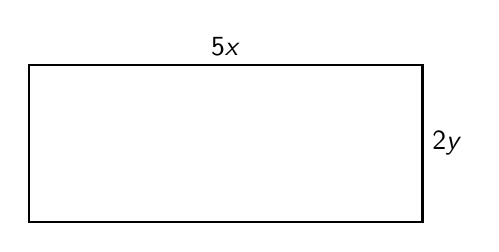
\begin{tikzpicture}[baseline=(current bounding box.north)]
  \draw[thick] (0,0) rectangle (5,2);
  \node[above] at (2.5,2) {$5x$};
  \node[right] at (5,1) {$2y$};
\end{tikzpicture}
\end{minipage}

\vspace{14pt}
\ealpara{\ealkeytr{Pole} \ealkeytr{prostokąta} wynosi $12a^2$. Zapisz trzy różne pary długości, jakie mogą mieć jego boki.}{The \ealkey{area} of a \ealkey{rectangle} is $12a^2$. Write down three different pairs of lengths that its sides could have.}
\qlabel The \ealkey{area} of a \ealkey{rectangle} is $12a^2$. Write down three different pairs of lengths that its sides could have.
\writeline\writeline

\vspace{10pt}
\ealpara{Zapisz \ealkeytr{wyrażenie} z czterema \ealkeytr{wyrazami}, które \ealkeytr{upraszcza} się do $5x-2y$.}{Write an \ealkey{expression} with four \ealkey{terms} that \ealkey{simplifies} to $5x-2y$.}
\qlabel Write an \ealkey{expression} with four \ealkey{terms} that \ealkey{simplifies} to $5x-2y$.
\writeline

\vspace{10pt}
\ealpara{Zapisz trzy różne mnożenia, które można \ealkeytr{uprościć} do $6a^2b$.}{Write three different multiplications that \ealkey{simplify} to $6a^2b$.}
\qlabel Write three different multiplications that \ealkey{simplify} to $6a^2b$.
\writeline

\end{document}